%% International Journal of Computational Intelligence Systems ---
%%%%%%%%%%%%%%%%%%%%%%%%%%%%%%%%%%%%%%%%%%%%%%%%%%%%%%%%%%%%%%%%%%%%%%%%%%%
\documentclass[11pt,twoside]{article}
\usepackage{ijcis}
%--------------------- ADDITIONAL PACKAGES HERE ---------------------------
\usepackage{lscape}
\usepackage{pdflscape}
\usepackage{setspace}
\usepackage{afterpage}
\usepackage{alltt}
%--------------------------------------------------------------------------
%
\def\labart{yourLabel}      % put a label from your choice here
%\Vol{1}                    % number of the Volume
%\Issue{1}                  % number of the issue
%\Month{January}            % month
%\Year{2008}                % year
%\received{...}
%\revised{...}
%
%---------------------------------------------------------------------------
\thispagestyle{empty}
%%------------------------- YOUR HEADINGS HERE -----------------------------
% Author's initials of first names+last names
\shortauthors{Pablo Cingolani, Jes\'us Alcal\'a-Fdez}
% Short title
\shorttitle{jFuzzyLogic}
%---------------------------------------------------------------------------
%
%---------------------- YOUR TITLE ----------------------------------------
\title{jFuzzyLogic: A Robust and Flexible Fuzzy-Logic Inference System Language Implementation}
%-------------------------- AUTHOR'S NAMES ----------------------------------
\author{%
Pablo Cingolani\,\up{1},
%\author{
Jes\'us Alcal\'a-Fdez\,\up{2}
}
%----------------------------- ADDRESSES ----------------------------------
\addresses\address{%
\\ \vspace*{0.05truein}
\up{2}
Department of Computer Science and Artificial Intelligence, University of Granada,\\
Research Center on Information and Communications Technology,\\
C/ Periodista Daniel Saucedo Aranda s/n,\\ 
Granada, 18071, Spain
\\ \vspace*{0.04truein}
E-mail: jalcala@decsai.ugr.es
}
%---------------------------------------------------------------------------
\pagestyle{myheadings}
\begin{document}
\label{\labart-FirstPage}

\maketitle
%-------------------------- ABSTRACT ---------------------------------------
\abstracts{%
This work introduces jFuzzyLogic, an open source library for fuzzy systems which allow us to design Fuzzy Logic Controllers supporting the standard for Fuzzy Control Programming published by the International Electrotechnical Commission. This library is written in Java and is available as open source from jfuzzylogic.sourceforge.net. The use of jFuzzyLogic is illustrated through the analysis of one case study.
% This paper introduces jFuzzyLogic, an open source library for fuzzy systems which allow us to design Fuzzy Logic Controllers supporting the standard for Fuzzy Control Programming 
% published by the International Electrotechnical Commission. This library is written in Java and is available as open source from jfuzzylogic.sourceforge.net. The use of jFuzzyLogic is 
% illustrated through the analysis of one case study.
}
\par\bigskip\par
%-------------------------- KEYWORDS ---------------------------------------
\keywords{Java Library, Fuzzy Logic Controller, IEC 61131-7, Open Source Software}

\vspace*{10pt}\textlineskip
%-------------------------- BEGIN BODY OF TEXT -----------------------------
\begin{multicols}{2}


\section{A case study}
\label{sec:cas}

We present an example of creating two FLC controllers with jFuzzyLogic. This case study is focused on the development of the wall following robot as explained in \cite{Mucientes2010}. Wall following behavior is well known in mobile robotics. It is frequently used for the exploration of unknown indoor environments and for the navigation between two points in a map. 

The main requirement of a good wall-following controller is to maintain a suitable distance from the wall that is being followed. The robot should also move as fast as possible, while avoiding sharp movements, making smooth and progressive turns and changes in velocity.

In our fuzzy control system, the input variables are: 
	i) normalized distances from the robot to the right ($RD$) and left walls ($DQ$); 
	ii) orientation with respect to the wall ($O$); and 
	iii) linear velocity ($V$). 

The output variables in this controller are the normalized linear acceleration ($LA$) and the angular velocity ($AV$). The linguistic partitions are shown in Figure~\ref{f:robotVars} which are comprised by linguistic terms with uniformly distributed triangular membership functions giving meaning to them.

\vspace*{10pt}
\centerline{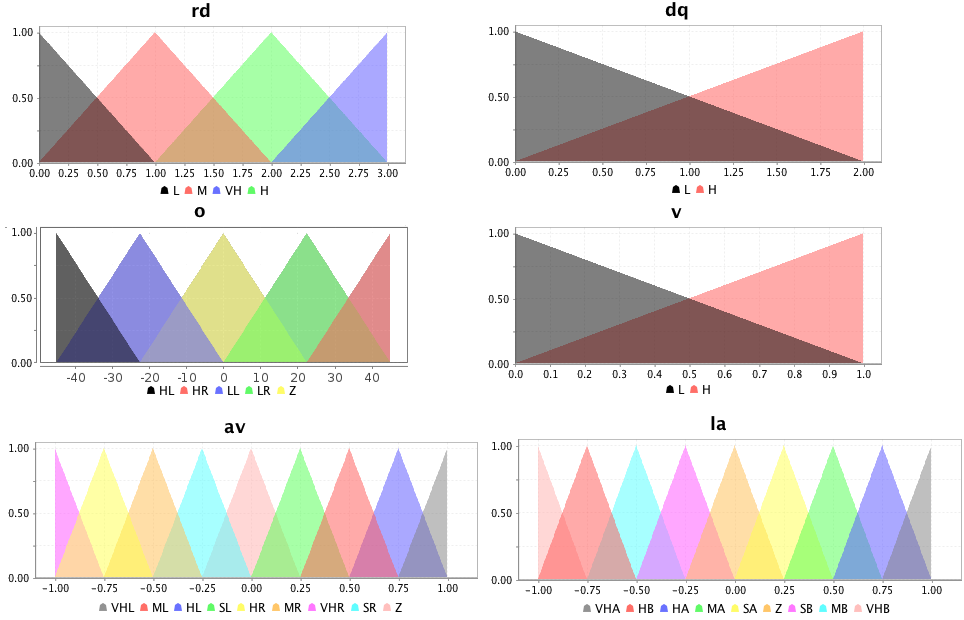
\includegraphics[width=3.1in]{./figs/robot_vars_2.png}}
\vspace*{10pt}
\fcaption{Membership functions for wall-following robot.}\label{f:robotVars}
\vspace*{10pt}

In order to implement the controller, the first step is to declare the input and output variables and to define the fuzzy sets. Variables are defined in \textit{VAR\_INPUT} and \textit{VAR\_OUTPUT} sections. Fuzzy sets are defined in \textit{FUZZIFY} blocks for input variables and \textit{DEFUZZIFY} blocks for output variables.

One \textit{FUZZIFY} block is used for each input variable. Each \textit{TERM} line within a \textit{FUZZIFY} block defines a linguistic term and its corresponding membership function.  In this example all membership functions are triangular, so they are defined using the \textit{'trian'} keyword, followed by three parameters defining left, center and right points (e.g. \textit{`trian 1 2 3'}).

Output variables define their membership functions within \textit{DEFUZZIFY} blocks. Linguistic terms and membership functions are defined using the \textit{TERM} keyword as previously described for input variables. In this case we also add parameters to select the defuzzyfication method. The statement \textit{'METHOD : COG'} indicates that we are using 'Center of gravity'. The corresponding Java code generated for the first step is as follows:

\vspace*{10pt}
\begin{scriptsize}
\begin{alltt}
VAR\_INPUT
	rd : REAL;			// Right distance
	dq : REAL;			// Distance quotient
	o  : REAL;			// Orientation. Note: 'or' is a reserved word
	v  : REAL;			// Velocity
END\_VAR

VAR\_OUTPUT
	la : REAL;			// Linear acceleration
	av : REAL;			// Angular velocity
END\_VAR

FUZZIFY rd
	TERM L  := trian 0 0 1;
	TERM M  := trian 0 1 2;
	TERM H  := trian 1 2 3;
	TERM VH := trian 2 3 3;
END\_FUZZIFY

FUZZIFY dq
	TERM L := trian 0 0 2;
	TERM H := trian 0 2 2;
END\_FUZZIFY

FUZZIFY o
	TERM HL := trian -45 -45 -22.5;
	TERM LL := trian -45 -22.5 0;
	TERM Z  := trian -22.5 0 22.5;
	TERM LR := trian 0 22.5 45;
	TERM HR := trian 22.5 45 45;
END\_FUZZIFY

FUZZIFY v
	TERM L := trian 0 0 1;
	TERM H := trian 0 1 1;
END\_FUZZIFY

DEFUZZIFY la
	TERM VHB := trian -1 -1 -0.75;
	TERM HB  := trian -1 -0.75 -0.5;
	TERM MB  := trian -0.75 -0.5 -0.25;
	TERM SB  := trian -0.5 -0.25 0;
	TERM Z   := trian -0.25 0 0.25;
	TERM SA  := trian 0 0.25 0.5;
	TERM MA  := trian 0.25 0.5 0.75;
	TERM HA  := trian 0.5 0.75 1;
	TERM VHA := trian 0.75 1 1;
	METHOD : COG;			// Center of Gravity
	DEFAULT := 0;
END\_DEFUZZIFY

DEFUZZIFY av
	TERM VHR := trian -1 -1 -0.75;
	TERM HR  := trian -1 -0.75 -0.5;
	TERM MR  := trian -0.75 -0.5 -0.25;
	TERM SR  := trian -0.5 -0.25 0;
	TERM Z   := trian -0.25 0 0.25;
	TERM SL  := trian 0 0.25 0.5;
	TERM ML  := trian 0.25 0.5 0.75;
	TERM HL  := trian 0.5 0.75 1;
	TERM VHL := trian 0.75 1 1;
	METHOD : COG;
	DEFAULT := 0;
END\_DEFUZZIFY
\end{alltt}
\end{scriptsize}

\vspace*{10pt}
These membership functions can be plotted by running jFuzzyLogic with the FCL file generated as argument (e.g. \texttt{java -jar jFuzzyLogic.jar robotCOR.fcl}). 
The corresponding FCL file for this case study is available for download as one of the examples provided in jFuzzyLogic package (\texttt{jfuzzylogic.sourceforge.net}).

The second step is to define the rules used for inference. They are defined in \textit{RULEBLOCK} statements. For the wall-following robot controller, we used 'minimum' connection method (\textit{AND : MIN}), minimum activation method (\textit{ACT : MIN}), and maximum accumulation method (\textit{ACCU : MAX}).  We implemented the rule bases generated in~\cite{mucientes2009learning} by the methods COR~\cite{Casillas02} and WCOR~\cite{Alc06}. Each entry in the rule bases was converted to a single FCL rule. Within each rule, the antecedent (i.e. the \textit{IF} part) is composed of the input variables connected by \textit{`AND'} operators. Since there are more than one output variable, we can specify multiple consequents (i.e. \textit{THEN} part) separated by semicolons. Finally, we add the desired weight using the \textit{`with'} keyword followed by the weight. This completes the implementation of a controller for a wall-following robot using FCL and jFuzzyLogic. The Java codes generated for COR and WCOR are the following:

\vspace*{10pt}
COR:
\begin{scriptsize}
\begin{alltt}
RULEBLOCK rules
AND  : MIN;			// Use 'min' for 'and' (also implicit use 
            //'max' for 'or' to fulfill DeMorgan's Law)
ACT  : MIN;			// Use 'min' activation method
ACCU : MAX;			// Use 'max' accumulation method

RULE 01: IF rd is L and dp is L and o is HL
    and v is L THEN la is VHB, av is VHR with 1.0;
RULE 02: IF rd is L and dp is L and o is LL
    and v is L THEN la is VHB, av is VHR with 1.0;
RULE 01: IF rd is L and dp is L and o is Z
    and v is L THEN la is MB, av is VHL with 1.0;
RULE 03: IF rd is L and dp is L and o is Z
     and v is H THEN la is VHB, av is HR with 1.0;
RULE 04: IF rd is L and dp is L and o is LR
    and v is L THEN la is SB, av is HL with 1.0;
RULE 05: IF rd is L and dp is L and o is HR
    and v is L THEN la is MB, av is VHL with 1.0;
RULE 06: IF rd is L and dp is L and o is HR
     and v is H THEN la is VHB, av is Z with 1.0;
RULE 07: IF rd is L and dq is H and o is HL
    and v is L THEN la is HB, av is VHR with 1.0;
RULE 08: IF rd is L and dq is H and o is HL
    and v is H THEN la is VHB, av is VHR with 1.0;
RULE 09: IF rd is L and dq is H and o is LL
    and v is L THEN la is MA, av is Z with 1.0;
RULE 10: IF rd is L and dq is H and o is LL
    and v is H THEN la is VHB, av is HR with 1.0;
RULE 11: IF rd is L and dq is H and o is Z
    and v is L THEN la is SA, av is VHL with 1.0;
RULE 12: IF rd is L and dq is H and o is Z
    and v is H THEN la is VHB, av is SR with 1.0;
RULE 13: IF rd is L and dq is H and o is LR
    and v is L THEN la is SB, av is VHL with 1.0;
RULE 14: IF rd is L and dq is H and o is LR
    and v is H THEN la is VHB, av is VHL with 1.0;
RULE 15: IF rd is L and dq is H and o is HR
    and v is L THEN la is VHB, av is VHL with 1.0;
RULE 16: IF rd is M and dp is L and o is HL
    and v is L THEN la is VHB, av is VHR with 1.0;
RULE 17: IF rd is M and dp is L and o is HL
    and v is H THEN la is VHB, av is VHR with 1.0;
RULE 18: IF rd is M and dp is L and o is LL
    and v is L THEN la is SA, av is VHR with 1.0;
RULE 19: IF rd is M and dp is L and o is LL
    and v is H THEN la is HB, av is VHR with 1.0;
RULE 20: IF rd is M and dp is L and o is Z
    and v is L THEN la is HA, av is VHR with 1.0;
RULE 21: IF rd is M and dp is L and o is LR
    and v is L THEN la is HA, av is HL with 1.0;
RULE 22: IF rd is M and dp is L and o is LR
    and v is H THEN la is VHB, av is Z with 1.0;
RULE 23: IF rd is M and dp is L and o is HR
    and v is L THEN la is VHA, av is VHL with 1.0;
RULE 24: IF rd is M and dp is L and o is HR
    and v is H THEN la is VHB, av is VHL with 1.0;
RULE 25: IF rd is M and dq is H and o is HL
    and v is L THEN la is SB, av is VHR with 1.0;
RULE 26: IF rd is M and dq is H and o is HL
    and v is H THEN la is VHB, av is VHR with 1.0;
RULE 27: IF rd is M and dq is H and o is LL
    and v is L THEN la is MA, av is VHR with 1.0;
RULE 28: IF rd is M and dq is H and o is Z
    and v is L THEN la is VHA, av is Z with 1.0;
RULE 29: IF rd is M and dq is H and o is Z
    and v is H THEN la is Z, av is Z with 1.0;
RULE 30: IF rd is M and dq is H and o is LR
    and v is L THEN la is MA, av is VHL with 1.0;
RULE 31: IF rd is M and dq is H and o is LR
    and v is H THEN la is VHB, av is VHL with 1.0;
RULE 32: IF rd is M and dq is H and o is HR
    and v is L THEN la is VHB, av is VHL with 1.0;
RULE 33: IF rd is M and dq is H and o is HR
    and v is H THEN la is VHB, av is VHL with 1.0;
RULE 34: IF rd is H and dp is L and o is HL
    and v is L THEN la is VHB, av is VHR with 1.0;
RULE 35: IF rd is H and dp is L and o is HL
    and v is H THEN la is VHB, av is VHR with 1.0;
RULE 36: IF rd is H and dp is L and o is LL
    and v is L THEN la is VHA, av is VHR with 1.0;
RULE 37: IF rd is H and dp is L and o is LL
    and v is H THEN la is VHB, av is VHR with 1.0;
RULE 38: IF rd is H and dp is L and o is Z
    and v is L THEN la is VHA, av is VHR with 1.0;
RULE 39: IF rd is H and dp is L and o is Z
    and v is H THEN la is Z, av is VHR with 1.0;
RULE 40: IF rd is H and dp is L and o is LR
    and v is L THEN la is VHA, av is VHR with 1.0;
RULE 41: IF rd is H and dp is L and o is HR
    and v is H THEN la is Z, av is HL with 1.0;
RULE 42: IF rd is H and dq is H and o is HL
    and v is L THEN la is VHB, av is VHR with 1.0;
RULE 43: IF rd is H and dq is H and o is HL
    and v is H THEN la is VHB, av is VHR with 1.0;
RULE 44: IF rd is H and dq is H and o is LL
    and v is L THEN la is VHA, av is VHR with 1.0;
RULE 45: IF rd is H and dq is H and o is LL
    and v is H THEN la is VHB, av is VHR with 1.0;
RULE 46: IF rd is H and dq is H and o is Z
    and v is L THEN la is VHA, av is VHR with 1.0;
RULE 47: IF rd is H and dq is H and o is Z
    and v is H THEN la is MA, av is VHR with 1.0;
RULE 48: IF rd is H and dq is H and o is LR
    and v is L THEN la is VHA, av is VHR with 1.0;
RULE 49: IF rd is H and dq is H and o is HR
    and v is L THEN la is VHA, av is HR with 1.0;
RULE 50: IF rd is H and dq is H and o is HR
    and v is H THEN la is Z, av is HL with 1.0;
RULE 51: IF rd is VH and dp is L and o is HL
    and v is L THEN la is VHB, av is VHR with 1.0;
RULE 52: IF rd is VH and dp is L and o is HL
    and v is H THEN la is VHB, av is VHR with 1.0;
RULE 53: IF rd is VH and dp is L and o is Z
    and v is L THEN la is VHA, av is VHR with 1.0;
RULE 54: IF rd is VH and dp is L and o is LR
    and v is L THEN la is VHA, av is VHR with 1.0;
RULE 55: IF rd is VH and dp is L and o is LR
    and v is H THEN la is MA, av is VHR with 1.0;
RULE 56: IF rd is VH and dp is L and o is HR
    and v is L THEN la is VHA, av is VHR with 1.0;
RULE 57: IF rd is VH and dq is H and o is HL
    and v is L THEN la is VHB, av is VHR with 1.0;
RULE 58: IF rd is VH and dq is H and o is LL
    and v is L THEN la is VHB, av is VHR with 1.0;
RULE 59: IF rd is VH and dq is H and o is Z
    and v is L THEN la is VHA, av is VHR with 1.0;
RULE 60: IF rd is VH and dq is H and o is Z
    and v is H THEN la is MA, av is VHR with 1.0;
RULE 61: IF rd is VH and dq is H and o is LR
    and v is L THEN la is VHA, av is VHR with 1.0;
RULE 62: IF rd is VH and dq is H and o is HR
    and v is L THEN la is VHA, av is VHR with 1.0;
\end{alltt}
\end{scriptsize}
\vspace*{10pt}



\vspace*{10pt}
WCOR:
\begin{scriptsize}
\begin{alltt}
RULEBLOCK rules
AND  : MIN;			// Use 'min' for 'and' (also implicit use 
            //'max' for 'or' to fulfill DeMorgan's Law)
ACT  : MIN;			// Use 'min' activation method
ACCU : MAX;			// Use 'max' accumulation method

RULE 01: IF rd is  L and dq is L and o is LL 
    and v is L THEN la is VHB , av is VHR with 0.4610;
RULE 02: IF rd is  L and dq is L and o is LL 
    and v is H THEN la is VHB , av is VHR with 0.4896;
RULE 03: IF rd is  L and dq is L and o is  Z 
    and v is L THEN la is   Z , av is  MR with 0.6664;
RULE 04: IF rd is  L and dq is L and o is  Z 
    and v is H THEN la is  HB , av is  SR with 0.5435;
RULE 05: IF rd is  L and dq is H and o is LL 
    and v is L THEN la is  MA , av is  HR with 0.7276;
RULE 06: IF rd is  L and dq is H and o is  Z 
    and v is L THEN la is  MA , av is  HL with 0.4845;
RULE 07: IF rd is  L and dq is H and o is  Z 
    and v is H THEN la is  HB , av is  ML with 0.5023;
RULE 08: IF rd is  L and dq is H and o is LR 
    and v is H THEN la is VHB , av is VHL with 0.7363;
RULE 09: IF rd is  L and dq is H and o is HR 
    and v is L THEN la is VHB , av is VHL with 0.9441;
RULE 10: IF rd is  M and dq is L and o is  Z 
    and v is H THEN la is  SA , av is  HR with 0.3402;
RULE 11: IF rd is  M and dq is L and o is LR 
    and v is H THEN la is   Z , av is VHL with 0.4244;
RULE 12: IF rd is  M and dq is L and o is HR 
    and v is L THEN la is  SA , av is  HL with 0.5472;
RULE 13: IF rd is  M and dq is L and o is HR 
    and v is H THEN la is  MB , av is VHL with 0.4369;
RULE 14: IF rd is  M and dq is H and o is HL 
    and v is L THEN la is   Z , av is VHR with 0.1770;
RULE 15: IF rd is  M and dq is H and o is HL 
    and v is H THEN la is VHB , av is VHR with 0.4526;
RULE 16: IF rd is  M and dq is H and o is LL 
    and v is H THEN la is  SA , av is VHR with 0.2548;
RULE 17: IF rd is  M and dq is H and o is  Z 
    and v is L THEN la is  HA , av is   Z with 0.2084;
RULE 18: IF rd is  M and dq is H and o is LR 
    and v is L THEN la is  HA , av is VHL with 0.6242;
RULE 19: IF rd is  M and dq is H and o is LR 
    and v is H THEN la is  SA , av is VHL with 0.3779;
RULE 20: IF rd is  M and dq is H and o is HR 
    and v is L THEN la is   Z , av is VHL with 0.6931;
RULE 21: IF rd is  M and dq is H and o is HR 
    and v is H THEN la is VHB , av is VHL with 0.7580;
RULE 22: IF rd is  H and dq is L and o is  Z 
    and v is L THEN la is  HA , av is VHR with 0.5758;
RULE 23: IF rd is  H and dq is L and o is LR 
    and v is H THEN la is  SA , av is  MR with 0.2513;
RULE 24: IF rd is  H and dq is L and o is HR 
    and v is L THEN la is  HA , av is VHL with 0.5471;
RULE 25: IF rd is  H and dq is L and o is HR 
    and v is H THEN la is  SA , av is  HL with 0.5595;
RULE 26: IF rd is  H and dq is H and o is HL 
    and v is L THEN la is VHB , av is VHR with 0.9999;
RULE 27: IF rd is  H and dq is H and o is HL 
    and v is H THEN la is VHB , av is VHR with 0.9563;
RULE 28: IF rd is  H and dq is H and o is LL 
    and v is L THEN la is  HA , av is VHR with 0.9506;
RULE 29: IF rd is  H and dq is H and o is  Z 
    and v is L THEN la is  HA , av is VHR with 0.4529;
RULE 30: IF rd is  H and dq is H and o is  Z 
    and v is H THEN la is  SA , av is VHR with 0.2210;
RULE 31: IF rd is  H and dq is H and o is LR 
    and v is L THEN la is  HA , av is  MR with 0.3612;
RULE 32: IF rd is  H and dq is H and o is LR 
    and v is H THEN la is  SA , av is  MR with 0.2122;
RULE 33: IF rd is  H and dq is H and o is HR 
    and v is L THEN la is  HA , av is  HL with 0.7878;
RULE 34: IF rd is  H and dq is H and o is HR 
    and v is H THEN la is  SA , av is VHL with 0.3859;
RULE 35: IF rd is VH and dq is L and o is LR 
    and v is L THEN la is  HA , av is VHR with 0.5530;
RULE 36: IF rd is VH and dq is L and o is HR 
    and v is L THEN la is  HA , av is  HR with 0.4223;
RULE 37: IF rd is VH and dq is L and o is HR 
    and v is H THEN la is  SA , av is  HR with 0.3854;
RULE 38: IF rd is VH and dq is H and o is LL 
    and v is L THEN la is  HA , av is VHR with 0.0936;
RULE 39: IF rd is VH and dq is H and o is LR 
    and v is L THEN la is  HA , av is VHR with 0.7325;
RULE 40: IF rd is VH and dq is H and o is LR 
    and v is H THEN la is  SA , av is VHR with 0.5631;
RULE 41: IF rd is VH and dq is H and o is HR 
    and v is L THEN la is  HA , av is  HR with 0.5146;
END\_RULEBLOCK
\end{alltt}
\end{scriptsize}
\vspace*{10pt}

\vspace*{10pt}
The corresponding Java code that use jFuzzyLogic for running the FCL generated for COR will be:
\\
\begin{scriptsize}
\begin{alltt}
public class TestRobotCOR \{
  public static void main(String[] args) 
  throws Exception \{
    FIS fis = FIS.load("fcl/robotCOR.fcl", true);
    FunctionBlock fb = fis.getFunctionBlock(null);
    // Set inputs
    fb.setVariable("rd", 0.3); 
    fb.setVariable("dp", 1.25);
    fb.setVariable("o", 2.5); 
    fb.setVariable("v", 0.6);
    // Evaluate
    fb.evaluate(); 
    // Get output
    double la = fb.getVariable("la").getValue());
    double av = fb.getVariable("av").getValue());
  \}
\}
\end{alltt}
\end{scriptsize}

\section{Conclusions}
\label{sec:con}

In this paper, we have described jFuzzyLogic, an open source Java library for fuzzy systems which allow us to design FLCs following the standard IEC 61131.
It allows us to reduce programming work and extend the range of possible users applying fuzzy systems and FLCs.

We have shown a case study to illustrate the use of jFuzzyLogic. 
In this case, we developed an FLC controller for wall-following behavior in a robot.
The example shows how FCL can be used to easily implement fuzzy logic systems.

The jFuzzyLogic software package is continuously being updated and improved. 
At the moment, we are developing an implementation of a C/C++ compiler for fuzzy inference systems. 
This will allow easy implementation with embedded control systems using different processors.

\section*{Acknowledgments}
jFuzzyLogic was designed and developed by P. Cingolani. He is supported in part by McGill Uninversity, Genome Quebec. J. Alcala-Fdez is supported by the Spanish Ministry of Education and Science under Grant TIN2011-28488 and the Andalusian Government under Grant P10-TIC-6858. We would like to thank R. Sladek and M. Blanchette for their comments. Special thanks to P.J. Leonard for his contributions to the project.


\section*{References}
\bibliographystyle{unsrt}
\bibliography{CingolaniAlcala-Fdez-IJCIS2012}
\end{multicols}
\end{document}
